% !TeX root = ../main.tex
% Add the above to each chapter to make compiling the PDF easier in some editors.

\chapter{Implementation}\label{chapter:implementation}
In order to test the effects of the modifications and simplifications made in chapter \ref{chapter:navier_stokes}, and the effects of discretization described in chapter \ref{chapter:discretization}, everything discussed was implemented using a custom framework written in Python 3 with aid of the numpy-library.
The architecture of this framework will be described in this chapter.

\section{Design}
The framework was created keeping the design principle of modularity in mind.
This has several advantages.
First, it becomes possible to test and verify every component of the framework individually.
Second, it becomes easier to fulfill the goal of the framework, namely to test every possible configuration of simplifications and discretizations.
Modularizing these simplifications and discretizations makes it possible to switch between them easily.
\\
The functionality of the framework can be separated into two components. 
The first component is responsible for generating the data through either simulation or usage of analytic solutions.
This component is called Generator.
\\
The second component can then be used to evaluate the generated data, by using its error tracking and visualization\footnote{using matplotlib} capabilities.
This component is called Evaluator.

\subsection*{Generator}
Focusing on the data-generating component, its functionality was split up as follows:
\begin{itemize}
\item differential operators, modeled by functions. 
These functions take in a vector representing a scalar or vector field (represented by a numpy-array), perform their respective operation on it, and return the result of the operation.
\item storing the system state in instances of the class \texttt{State}.
This class wraps a numpy-array storing the state variables, and the names of the all axes and variables.
\item differential equations, modeled by classes inheriting from the abstract class \texttt{TimeDerivative}.
When called and given an instance of \texttt{State}, objects of the \texttt{TimeDerivative} class calculate the time derivative given the current state, by applying the diagnostic equations of their respective differential equation to it.
\item integrators, modeled by classes inheriting from the abstract class \texttt{Integrator}.
During instantiation they receive an initial state and a differential equation (in the form of an \texttt{TimeDerivative} instance), which they are supposed to integrate, using a specified step size.
Every time an instance of \texttt{Integrator} is called it will integrate its differential equation by one step, advance its internal time by one step, and output the modified \texttt{State} instance.
\item analytic solutions to differential equations, modeled by classes inheriting from the abstract class \texttt{Solution}.
As these solutions are analytic, any time t can be specified, and an instance of \texttt{Solution} will output the state of the system modeled by its differential equation.
In order to be more similar to \texttt{Integrator} classes, they also contain an internal timer, which can be advanced by calling the instance of \texttt{Solution} without specifying a time t.
\end{itemize}
Using this separation into classes fulfills the objective of modularity.
For one, one \texttt{Integrator} class can be replaced for another without affecting other components of the program.
The same goes for different implementations of the same differential operators.
Second, for a given differential equation, it is possible to implement several different test scenarios or analytic solutions, by representing each by its own \texttt{Solution} class.
Last, it is possible to change the differential equation being simulated by changing the \texttt{TimeDerivative} class.
\\
As already mentioned above, as another design step taken for better readability, any class which repeatedly outputs new data was implemented as an iterator.
This includes all classes inheriting from \texttt{Integrator} and \texttt{Solution}, as they both generate new output for every iteration.
Using iterators makes code using repeated data-generation more compact and readable.

\subsection*{Evaluator}
The evaluator component builds on the premise that there is a solution (coming from a \texttt{Solution} object) and a calculated result (coming from an \texttt{Integrator} object).
Both calculated results and solutions are a discrete series of system states over time.
Within the program they are represented by a discrete series of \texttt{State} objects at monotonically increasing timestamps.
Of course there may be some differences between the solution and the calculated result, which will subsequently be called errors.
\\
The functionality of the component was split up as follows:
\begin{itemize}
\item the \texttt{ErrorTracker} class, which is used to store a series of errors, along with some kind of labeling (e.g. time, or spacial resolution).
Example: To store errors over time, every time step, an instance of \texttt{ErrorTracker} is given a timestamp as a label, the calculated result, and the solution at that timestamp.
From this it calculates the error (using a norm of the programmers choice) and stores it together with the timestamp.
\item the \texttt{ErrorIntegrator} class, which also calculates the error whenever it is given a calculated result and a solution, but then adds it its memorized total error, instead of storing it individually.
\item the \texttt{WindowManager} class is used for displaying both instances of \texttt{State} and of \texttt{ErrorTracker} visually.
Errors can be displayed both on a logarithmic and on an ordinary scale.
\\
For displaying \texttt{State} objects, the class also provides some functionality to apply a custom transformation to the data to be displayed, before displaying it.
\\
Example: When simulating, $\text{ln}p$ can be a diagnostic variable. In order to display $p$ instead of $\text{ln}p$, it needs to transformed through exponentiation first.
\end{itemize}

\subsection{Operators}
The smallest units of the framework are the operators.
Two categories of operators have been implemented: averaging operators, and the differential operators discussed in section \ref{section:diff_op}.\\
The averaging operators follow the naming scheme:
\\
\texttt{[operation abbreviation]\_e[error order]}
\\
where the error order indicates how many neighboring variables are taken into account when calculating the local average.
When considering a high spacial resolution, using more neighboring variables will make the estimation more accurate.
\\
The differential operators follow the naming scheme:
\\
\texttt{[operation abbreviation]\_n[operator order]\_e[error order]}
\\ 
where the \texttt{operator order} can either be \texttt{1} for the first order derivative, or \texttt{2} for the second order derivative (also known as the laplacian).
The error order \texttt{e} is the exponent of $h$ in the error term $\mathcal{O}(h^\texttt{e})$ (see section \ref{section:diff_op}).

\subsection{Class Structure and Information Flow}
The interaction between the different types of classes is visualized in fig. \ref{UML_diagram}.

\begin{figure}[!h]
	\makebox[\textwidth]{ 
  		 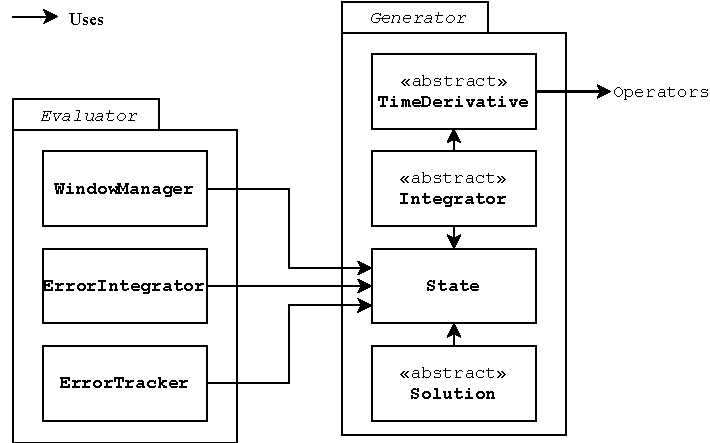
\includegraphics[width=.8\textwidth]{figures/UML.pdf}}
    \caption{UML-Style-Diagram}
    \label{UML_diagram}
\end{figure}

All communication between classes is done by passing references to \texttt{State}-objects.
As \texttt{State} objects can take up a lot of space in memory, passing them by reference is better than passing copies of them.
For the same reason, whenever possible, \texttt{State}-objects are reused to avoid overcrowding memory.
\\
During execution, both the \texttt{Integrator}- and the \texttt{Solution}-instance contain one \texttt{State}-object each.
Whenever new information is requested from them, they generate it, and return a reference to their internal \texttt{State}-object.
Now, the program that requested the information can use the \texttt{State}-objects.
To this end the Evaluator components can be used.

\subsection{Usage of the Framework}
Having established the framework with its abstract classes, in this section the way it is used is described.
As was foreseen during design, there are multiple implementations of the abstract \texttt{Integrator}, namely implementations of RK1 (explicit Euler), RK2 (explicit Heun), RK4, and an implementation of an exponential integrator.
All of them can be found in the same folder.
\\
The remaining abstract classes are \texttt{TimeDerivative} and \texttt{Solution}.
Both of them are dependent on the differential equation to be simulated, and on the way it is simulated, i.e. different spacial discretizations/grids require new implementations of both \texttt{TimeDerivative} and \texttt{Solution}.
For this reason there is a separate folder for each differential equation to be analyzed.
Within each folder an appropriate implementation of \texttt{TimeDerivative} and \texttt{Solution} can be found.
\\
To now put everything together, the modus operandi is as follows:
First, an initial state of the system must be defined.
If the calculated result should be compared against an analytic solution, the initial state can be gained by first creating an instance of \texttt{Solution}, and then asking it for the system state at time $0$.
Otherwise one can directly create an instance of \texttt{State} and set its initial conditions manually.
\\
Next, an instance of \texttt{TimeDerivative} must is created.
Both this instance and the instance of \texttt{State} containing the starting conditions of the system are necessary to create an instance of \texttt{Integrator}.
\\
Now, depending on what the aim of the simulation is, the appropriate instances from the Evaluator components can be instantiated, which concludes the setup.
\\
As both \texttt{Integrator} and \texttt{Solution} are implemented as iterators, the system can simulated by using a simple \texttt{for}-loop.
As an iterator, \texttt{Integrator} will return the calculated result, and \texttt{Solution} will return the analytic result.
This means that within the \texttt{for}-loop the programmer has access to the accurate result, the analytic result, and can now perform any further necessary operations on those results.
\\
For some of the most common operations a programmer might want to do within the \texttt{for}-loop, a function performing the entire setup has been preimplemented in the \texttt{run\_ utils.py} file.
\\
Another helpful preimplementation is that of the numerical reference solution.
It can be used whenever no analytic solution is known, but a reference solution is still required.
In this case, a reference solution is created by simulating the differential equation using RK4 and doing very small time-steps.
To avoid having to re-calculate this, the result of this time-intensive simulation is stored to the disk.

\section{Testing}\label{sec:testing}
While it is not possible to mathematically prove that the implementation is without fault, the next best thing is exhaustive testing.
For this framework testing usually entails checking the outputs of the components against a reference solution, which was found separately.
This reference solution is usually analytic in nature and has to be derived through manual calculation.
\\
The approach taken to test the framework was bottom-up, i.e. first, the smallest possible components were tested in isolation, then, components using only tested sub-components could be tested, too.
In the following the tests for the Generator components are described.

\subsection{Operators}
In the case of this framework the smallest component are the operators.
They were tested using operations simple enough that a simple analytic expression exists.
Then the result of the numerical operator was compared against this analytic expression.
For the averaging operators this step was sufficient.
\\
In order to further verify the derivative operators, the order of the error was also checked, i.e. after changing the spacial resolution by a factor of $a$, an operator of the $n$-th error order was expected to reduce its error by a factor of $a^n$.

\subsection{Integrators}
In order to test the integrators separately from the differential operators, single-variable differential equations were used.
Having only one variable and no spacial dimension means spacial derivative operators do not have to be utilized.
For testing purposes four such differential equations for which analytic solutions exist, were implemented as subclasses of  \texttt{TimeDerivative} and \texttt{Solution}.
Having isolated the Integrator as the component to be tested (as much as possible), it is then run at different resolutions.
For Runge Kutta methods of order $n$ an increase in resolution by a factor of $a$ was expected to reduce error by a factor of $a^n$.
However, for exponential integrators this method fails, as exponential integrators are either accurate down to machine precision or wholly inaccurate.
For them, instead, a very small error was sufficient in order to complete the test.

\subsection{Differential Equations}
Having verified the implementation of both operators and integrators, the only component left to verify are the implementations of the differential equations in the form of \texttt{TimeDerivative}-implementations.
The process for this is similar to the previous sections: First, some analytic solution is found.
The breadth of this analytic solution can vary in its universality.
From analytic solutions describing the evolution of the system given any starting condition\footnote{which makes a numeric solutions redundant}, to analytic solutions describing the stationary solution of the system.
A stationary solution is a solution for which the state of the system does not change.
This solution is then implemented as a \texttt{Solution} class.
\\
After finding such an analytic solution, its initial state is given to an integrator (usually RK4), which uses the \texttt{TimeDerivative}-implementation to be tested in order to calculate its results independently from the analytic solution found.
\\
Now running both the analytic solution and the calculated simulation, these two results can be compared.
If the results are coinciding, chances are good the implementation of \texttt{TimeDerivative} was correct.
To further verify the solution, one can also vary the resolution with which RK4 is run.
If change in resolution by a factor of $a$ translates into a reduction in error by a factor of $a^4$, this is a good indicator that the solution described by \texttt{TimeDerivative} converges towards the analytic solution, which was found separately.

\subsection{Example}
TODO
\begin{itemize}
\item Lorenz-Grid
\item introduce used variables
\item show equivalence between symbolic math and code
\item show how to enforce boundary conditions
\end{itemize}